\section{Introduction}
\label{sec:introduction}

Botanix is an EVM-compatible layer 2 blockchain built on the Bitcoin network. Unlike most layer 2 systems that introduce new cryptocurrencies, Botanix employs a 1-to-1 peg with Bitcoin: users mint tokens by constructing a \textbf{pegin} through a verified Bitcoin transaction, and withdraw funds by constructing a \textbf{pegout} that burns tokens on Botanix and triggers a corresponding Bitcoin transaction.

Bitcoin's limited state introspection capabilities make it very hard to implement smart contracts that hold Bitcoin on behalf of external networks or validate their state transitions natively. This fundamental constraint drives the complexity addressed in this work: designing a secure, permissionless multisig system using FROST threshold signatures that can custody Bitcoin funds while maintaining the security and operational requirements of a production layer 2 network. The coordination complexity inherent to FROST, particularly its multi-round signing protocol and static membership requirements, fundamentally shapes our architectural decisions.

Botanix operates through three coordinated state layers, each producing cryptographic commitments that validators use to verify system-wide consistency:

\begin{itemize}
    \item \textbf{CometBFT}: Provides Byzantine Fault Tolerant consensus for block producer selection and transaction ordering
    \item \textbf{Application Layer}: Executes transactions and maintains deterministic EVM state, producing an EVM state commitment
    \item \textbf{Foundation Layer}: Coordinates multisig federation membership, pegout lifecycle management, and Bitcoin fork awareness, producing a Foundation state commitment
\end{itemize}

The Foundation Layer, which is the primary focus of this paper, addresses two key challenges: managing federation rotations despite FROST's static membership requirements, and tracking pegouts across Bitcoin's probabilistic finality model where chain reorganizations can "undo" previously confirmed transactions. These constraints motivate the two-tier federation architecture that balances security and operational flexibility.

\subsection{Document Structure}

This paper is organized into the following sections:

\begin{enumerate}
    \item \textbf{FROST Challenges \& Two-Tier Architecture}: Section \ref{sec:frost-challenge} describes the challenges inherent to the FROST protocol and motivates our two-tier federation system. Section \ref{sec:two-tier-federations} presents the architecture and analyzes the security-efficiency tradeoffs.
    \item \textbf{Pool Management}: Section \ref{sec:pool-management} presents the theory behind pegin and pegout allocation, defining how we balance the two-tier federation system securely and reliably.
          \begin{itemize}
              \item \textbf{Dynamic capacity targeting} (section \ref{sec:dynamic-capacity-target}): Maintains sufficient liquid funds in Tier 2 federations by adapting to pegout demand patterns
              \item \textbf{Real-time collateralization} (section \ref{sec:collateralization-level}): Ensures fund safety by tracking collateral backing for Tier 2 federations, mitigating risks from their smaller size
          \end{itemize}
    \item \textbf{Risk Assessment \& Lifecycle}: Section \ref{sec:risk-assessment} describes how DynaFed determines when new Tier 1 or Tier 2 federations must be established and how funds should be safely rotated to newly established federations.
          \begin{itemize}
              \item We define a reproducible risk metric that governs rotation urgency, favoring a conservative approach unless degradation is detected
          \end{itemize}
    \item \textbf{Pegout Proposals \& Bitcoin Finality}: Section \ref{sec:pegout-proposals} addresses the challenges of tracking pegout proposals once federation members construct Bitcoin L1 transactions.
          \begin{itemize}
              \item We examine how "executed" pegouts should be tracked across Bitcoin's probabilistic finality model and identify which assumptions cannot be made
              \item We leverage the UTXO-reuse property to prevent double-execution of pegouts in cases of orphaned Bitcoin blocks (where transactions return to mempool), proposal upgrades/fee bumps (section\ref{sec:pegout-proposal-upgrade}), or cancellations (section \ref{sec:pegout-proposal-cancellation})
              \item We present a lightweight Bitcoin fork awareness mechanism (section \ref{sec:bitcoin-fork-awareness}) that tracks pegout proposals across competing forks and orphaned blocks, enabling deterministic finality detection despite Bitcoin's probabilistic consensus
          \end{itemize}
    \item \textbf{Foundation Layer Integration}: Section \ref{sec:foundation-layer} describes the main component that coordinates all subsystems. The Foundation Layer interprets Botanix-specific consensus messages and orchestrates:
          \begin{itemize}
              \item Pegin and pegout routing decisions
              \item Dynamic capacity target and real-time collateralization calculations
              \item Risk metric computation and federation lifecycle management (construction, rotation, sunset)
              \item Bitcoin block and pegout proposal tracking with fork awareness
          \end{itemize}
\end{enumerate}

\begin{figure*}[t]
    \centering
    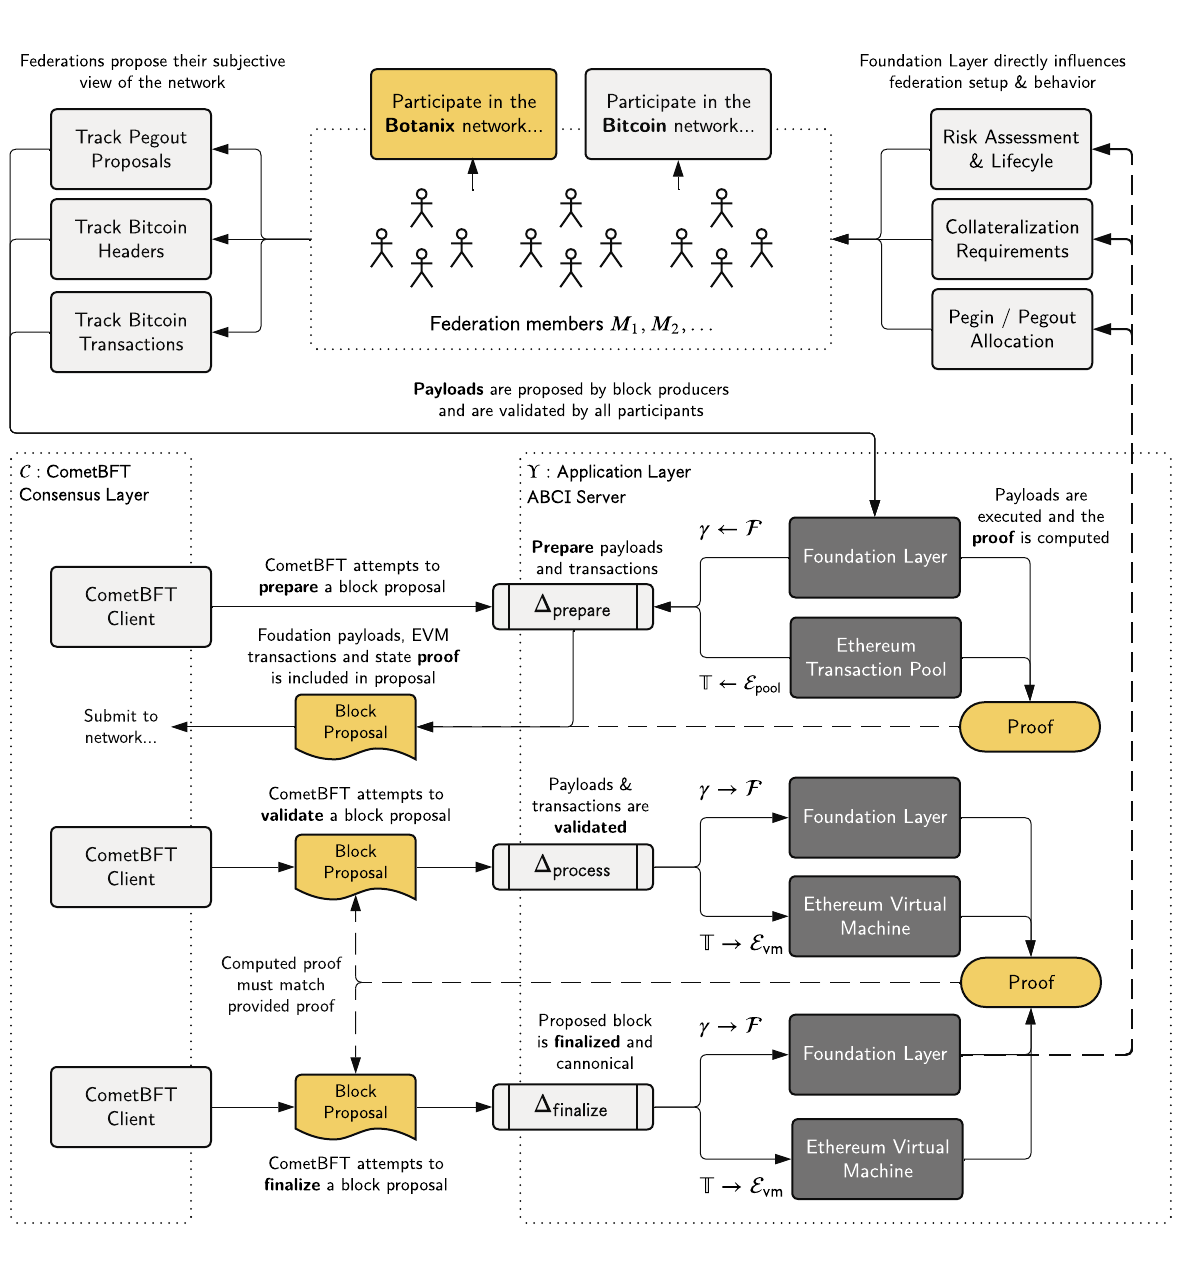
\includegraphics[width=\textwidth]{assets/dynafed_overview.png}
    \caption{DynaFed System Architecture}
    \label{fig:dynafed-overview}
\end{figure*}

\clearpage